\documentclass{article}[18pt]
\ProvidesPackage{format}
%Page setup
\usepackage[utf8]{inputenc}
\usepackage[margin=0.7in]{geometry}
\usepackage{parselines} 
\usepackage[english]{babel}
\usepackage{fancyhdr}
\usepackage{titlesec}
\hyphenpenalty=10000

\pagestyle{fancy}
\fancyhf{}
\rhead{Sam Robbins}
\rfoot{Page \thepage}

%Characters
\usepackage{amsmath}
\usepackage{amssymb}
\usepackage{gensymb}
\newcommand{\R}{\mathbb{R}}

%Diagrams
\usepackage{pgfplots}
\usepackage{graphicx}
\usepackage{tabularx}
\usepackage{relsize}
\pgfplotsset{width=10cm,compat=1.9}
\usepackage{float}

%Length Setting
\titlespacing\section{0pt}{14pt plus 4pt minus 2pt}{0pt plus 2pt minus 2pt}
\newlength\tindent
\setlength{\tindent}{\parindent}
\setlength{\parindent}{0pt}
\renewcommand{\indent}{\hspace*{\tindent}}

%Programming Font
\usepackage{courier}
\usepackage{listings}
\usepackage{pxfonts}

%Lists
\usepackage{enumerate}
\usepackage{enumitem}

% Networks Macro
\usepackage{tikz}


% Commands for files converted using pandoc
\providecommand{\tightlist}{%
	\setlength{\itemsep}{0pt}\setlength{\parskip}{0pt}}
\usepackage{hyperref}

% Get nice commands for floor and ceil
\usepackage{mathtools}
\DeclarePairedDelimiter{\ceil}{\lceil}{\rceil}
\DeclarePairedDelimiter{\floor}{\lfloor}{\rfloor}

% Allow itemize to go up to 20 levels deep (just change the number if you need more you madman)
\usepackage{enumitem}
\setlistdepth{20}
\renewlist{itemize}{itemize}{20}

% initially, use dots for all levels
\setlist[itemize]{label=$\cdot$}

% customize the first 3 levels
\setlist[itemize,1]{label=\textbullet}
\setlist[itemize,2]{label=--}
\setlist[itemize,3]{label=*}

% Definition and Important Stuff
% Important stuff
\usepackage[framemethod=TikZ]{mdframed}

\newcounter{theo}[section]\setcounter{theo}{0}
\renewcommand{\thetheo}{\arabic{section}.\arabic{theo}}
\newenvironment{important}[1][]{%
	\refstepcounter{theo}%
	\ifstrempty{#1}%
	{\mdfsetup{%
			frametitle={%
				\tikz[baseline=(current bounding box.east),outer sep=0pt]
				\node[anchor=east,rectangle,fill=red!50]
				{\strut Important};}}
	}%
	{\mdfsetup{%
			frametitle={%
				\tikz[baseline=(current bounding box.east),outer sep=0pt]
				\node[anchor=east,rectangle,fill=red!50]
				{\strut Important:~#1};}}%
	}%
	\mdfsetup{innertopmargin=10pt,linecolor=red!50,%
		linewidth=2pt,topline=true,%
		frametitleaboveskip=\dimexpr-\ht\strutbox\relax
	}
	\begin{mdframed}[]\relax%
		\centering
		}{\end{mdframed}}



\newcounter{lem}[section]\setcounter{lem}{0}
\renewcommand{\thelem}{\arabic{section}.\arabic{lem}}
\newenvironment{defin}[1][]{%
	\refstepcounter{lem}%
	\ifstrempty{#1}%
	{\mdfsetup{%
			frametitle={%
				\tikz[baseline=(current bounding box.east),outer sep=0pt]
				\node[anchor=east,rectangle,fill=blue!20]
				{\strut Definition};}}
	}%
	{\mdfsetup{%
			frametitle={%
				\tikz[baseline=(current bounding box.east),outer sep=0pt]
				\node[anchor=east,rectangle,fill=blue!20]
				{\strut Definition:~#1};}}%
	}%
	\mdfsetup{innertopmargin=10pt,linecolor=blue!20,%
		linewidth=2pt,topline=true,%
		frametitleaboveskip=\dimexpr-\ht\strutbox\relax
	}
	\begin{mdframed}[]\relax%
		\centering
		}{\end{mdframed}}
\lhead{CSys - Databases}
\usepackage{minted}

\begin{document}
\begin{center}
\underline{\huge SQL II}
\end{center}
\section{SQL Syntax}
Basis syntax of SQL queries:
\begin{minted}{sql}
SELECT [ALL|DISTINCT] column1[,column2,column3,...]
FROM table1[,table2,table3,...]
[WHERE "conditions"];
\end{minted}
\begin{itemize}
	\item The "conditions" in the WHERE clause can be:
	\begin{itemize}
		\item A comparison predicate (e.g. salary $>10000$)
		\item A range predicate (e.g. salary BETWEEN 10000 AND 30000)
		\item A set membership predicate (e.g. position IN('Manager','Worker'))
		\item A pattern matching predicate (e.g. address LIKE '\%Glaskow\%')
		\item Combinations of the above with AND and OR
	\end{itemize}
	\item But it can also be the result of another (independent) query (called subquery)
	\item Three types of subquery:
	\begin{enumerate}
		\item A single-value (scalar) subquery (single column \& single row )
		\begin{minted}{sql}
SELECT COUNT(*) AS myCount
FROM PropertyForRent
WHERE rent>350
		\end{minted}
		\item A multiple value subquery (one column \& multiple rows)
		\begin{minted}{sql}
SELECT staffNo
FROM Staff
WHERE position='Manager'
		\end{minted}
		\item A table subquery (multiple columns/rows)
		\begin{minted}{sql}
SELECT clientNo, viewDate
FROM Viewing
WHERE propertyNo='PG4' AND comment IS NULL
		\end{minted}
	\end{enumerate}
\end{itemize}
\section{Subquery}
\textit{List staff who work in branch at '163 Main St'}
\begin{minted}{sql}
SELECT staffNo, fName, IName, position
FROM Staff
WHERE branchNo=
	(SELECT branchNo
	 FROM Branch
	 WHERE street='163 Main St')
\end{minted}
\begin{itemize}
	\item The inner SELECT:
	\begin{itemize}
		\item Finds the branch number of the branch in 163 main street
		\item Only one such branch (with branchNo='B003')$\Rightarrow$ scalar subquery
	\end{itemize}
	\item The outer SELECT is equivalent with:
	\begin{minted}{sql}
SELECT staffNO, fName, IName, position
FROM Staff
WHERE branchNo='B003'
	\end{minted}
\end{itemize}
\newpage
\textit{List all staff whose salary is greater than the average salary, and show by how much}
\begin{itemize}
	\item If we know that the average salary is 17000, then:
	\begin{minted}{sql}
SELECT staffNo, fName, IName, position,	
	salary-17000 AS SalDiff
FROM Staff
WHERE salary>17000
	\end{minted}
	\item We cannot write "WHERE salary$>$AVG(salary)"
	\item Instead, we use a subquery
	\begin{minted}{sql}
SELECT staffNo, fName, IName, position
	salary-(SELECT AVG(salary) FROM Staff) AS SalDiff
FROM Staff
WHERE salary>(SELECT AVG(salary) FROM Staff)
	\end{minted}
\end{itemize}
\section{Nested Queries}
Example - (scalar subquery and multi-value subquery) - use of the operator IN:\\
\textit{List the properties that are handled by staff who work in the branch with the address '163 Main St'}
\begin{minted}{sql}
SELECT propertyNo, street, city, postcode, type, rooms, rent
FROM PropertyForRent
WHERE staffNo IN (SELECT staffNo
		FROM Staff
		WHERE branchNo=
			(SELECT branchNo
			 FROM branch
			 WHERE street='163 Main St'))
\end{minted}
\begin{itemize}
	\item From the innermost query outwards:
	\begin{itemize}
		\item The first query selects the branch number of the branch at 163 Main St
		\item The second selects the staff working at this branch
		\item Many staff $\Rightarrow$ in the outermost query we use IN ("=" is not possible)
	\end{itemize}
	\item In multi value subqueries:
	\begin{itemize}
		\item Use of the operator ANY (or SOME) before the subquery means the WHERE condition is true if it is satisfied by at least one value returned by the subquery
	\end{itemize}
\end{itemize}
\textit{Find all staff whose salary is larger than the salary of at least one member of staff at Branch B003}
\begin{minted}{sql}
SELECT staffNo, fName, IName, position, salary
FROM Staff
WHERE salary> SOME(SELECT salary
		   FROM Staff
		   WHERE branchNo='B003')
\end{minted}
An alternative would be:
\begin{minted}{sql}
WHERE salary>(SELECT MIN(salary)
	      FROM Staff
	      WHERE branchNo='B003')
\end{minted}
\section{Multi-Table Queries}
\begin{itemize}
	\item All examples so far have a major limitation: the whole information belongs to a single table
	\item We can extend queries to multiple tables either with subqueries that query different tables:\\
	\textit{List all Durham staff with salary greater than the average London-salary}
	\begin{minted}{sql}
SELECT staffNo, fName, IName, position
FROM DurhamStaff
WHERE salary>(SELECT AVG(salary) FROM LondonStaff)
	\end{minted}
	\item Or by using a join operation:
	\begin{itemize}
		\item Link data from two (or more) tables together (in a single query)
		\item Include more than one table in the FROM clause
		\item Separate these tables with a comma
	\end{itemize}
\end{itemize}
\section{Joins}
\begin{itemize}
	\item In joins, usually
	\begin{itemize}
		\item Include a WHERE clause to specify the joined columns
		\item We keep in the search only those rows which have the same values in the specified columns
		\item For clarity, in the SELECT clause, we can putt the table name before the column name (e.g. Staff.staffNo)
		\item Also possible to use an alias for a table in the FROM clause (useful for distinguishing column names in case of ambiguity)
		\item Alias is separated from table name with a space
	\end{itemize}
	\item Usually the syntax is
\begin{minted}{sql}
SELECT "list-of-columns"
WHERE table1,table2,...
WHERE "search conditions"
\end{minted}
\end{itemize}
\textit{List the details of all clients who have viewed a property, along with any comment supplied}
\begin{minted}{sql}
SELECT Client.ClientNo, Client.fname, Client.IName, Viewing.propertyNo, Viewing.comment
FROM Client, Viewing
WHERE Client.clientNo=Vieweing.clientNo
\end{minted}
Using an alias:
\begin{minted}{sql}
SELECT c.clientNo, c.fName, c.IName, v.propertyNo, v.comment
FROM Client c, Vieweing v
WHERE c.clientNo=v.clientNo
\end{minted}
This type of join is also known as a natural inner join:
\begin{itemize}
	\item Keeps the rows that coincide in the specified columns (in the WHERE clause)
	\item Ignores all rows that do not meet the join conditions
	\item The most common type of Join
\end{itemize}
\subsection{Three table Join}
\textit{For each branch, list staff who manage properties, including the city in which branch is located and the properties they manage}
\begin{minted}{sql}
SELECT b.branchNo, b.city, s.staffNo, s.fName, s.IName, p.propertyNo
FROM Branch b, Staff s, PropertyForRent p
WHERE b.branchNo=s.branchNo AND s.staffNo=p.staffNo
ORDER BY b.branchNo, s.staffNo, p.propertyNo
\end{minted}
An alternative formulation of this is
\begin{minted}{sql}
FROM (Branch b JOIN Staff s USING branchNo)
	JOIN PropertyForRent p USING staffNo
\end{minted}
\subsection{Inner Joins}
\begin{itemize}
	\item Instead of demanding the same column values in the matching columns we can demand different relations between the column values\\
	\textit{List all Durham-Staff who have salary 10\% more than some staff member in London}
\begin{minted}{sql}
SELECT dur.staffNo,dur.fName,dur.IName, dur.position, dur.salary
FROM DurhamSaff dur, LondonStaff lon
WHERE dur.salary>1.1*lon.salary
\end{minted}
	\item This type of join is an inner join:
	\begin{itemize}
		\item We add the term "natural", if we demand equality for the columns with the same name in the two tables (e.g. dur.salary=lon.salary)
		\item Inner joins still ignore all rows that do not meet the join conditions
	\end{itemize}
\end{itemize}
\subsection{Outer Joins}
\begin{itemize}
	\item Inner join: If one row of a table is unmatched, the row is omitted from the output table
	\item Outer join: It retains (some of) the rows that do not satisfy the join conditions
	\item Left outer join: It retains the rows of the left table that are unmatched with rows from the right table
	\item Right outer join: Retain the unmatched rows of the right table
	\item Full outer join: Retain the unmatched rows of both tables
\end{itemize}
\subsubsection{Example}
\begin{center}
	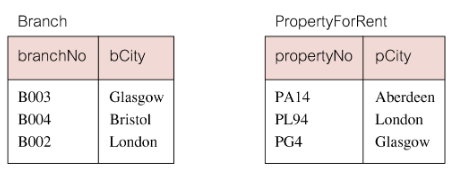
\includegraphics[scale=0.7]{example}
\end{center}
\textbf{Left outer Join}\\
\textit{List the branch offices which have any properties that are in the same city}
\begin{minted}{sql}
SELECT b.*,p.*
FROM Branch b LEFT JOIN PropertyForRent p
	ON b.bCity=p.pCity
\end{minted}
\begin{center}
	\includegraphics[scale=0.7]{"Left Outer"}
\end{center}
\begin{itemize}
	\item Includes the Bristol row of the left table unmatched with rows from the right table
	\item No rows corresponding to the properties in Aberdeen
\end{itemize}



\textbf{Right outer join}\\
\textit{List all properties and any branch offices that are in the same city}
\begin{minted}{sql}
SELECT b.*,p.*
FROM Branch b RIGHT JOIN PropertyForRent p
	ON b.bCity=p.pCity
\end{minted}
\begin{center}
	\includegraphics[scale=0.7]{"Right Outer"}
\end{center}
\begin{itemize}
	\item Includes the Aberdeen-row of the right table unmatched with rows from the left table
	\item No rows corresponding to branches in Bristol
\end{itemize}
\textbf{Full outer join}
\textit{List the branch offices and properties that are in the same city, along with any unmatched branches or properties}
\begin{minted}{sql}
SELECT b.*,p.*
FROM Branch b FULL JOIN PropertyForRent p
	ON b.bCity=p.pCity
\end{minted}
\begin{center}
	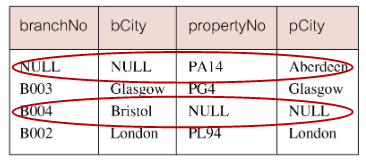
\includegraphics[scale=0.7]{Full}
\end{center}
\section{Database Updates}
Three SQL statements for modifying the contents of the (existing) tables in the database
\begin{itemize}
	\item \texttt{INSERT}: adds new rows of data into the table
	\begin{minted}{sql}
			INSERT INTO TableName [columnList]
			VALUES (data ValueList)
	\end{minted}
	\item \texttt{UPDATE}: Modifies existing data in a table
	\begin{minted}{sql}
			UPDATE TableName
			SET columnName1=dataValue1[,columnName2=dataValue2]
			[WHERE searchCondition]
	\end{minted}
	\item \texttt{DELETE}: Removes rows of data from a table
	\begin{minted}{sql}
			DELETE FROM TableName
			[WHERE searchCondition]
	\end{minted}
\end{itemize}
\section{Data Definition Language Overview}
Basic commands
\begin{itemize}
	\item \texttt{CREATE}: create a new table
	\begin{itemize}
		\item Assign a name to the table and define the names and domains of each of the columns in the table
	\end{itemize}
	\item \texttt{ALTER}: Amend the relation schema (i.e. table structure)
	\begin{itemize}
		\item If it is necessary to change the structure of a table because of design error, or just because the design has changed
	\end{itemize}
	\item Specify integrity and referential constraints
	\begin{itemize}
		\item \texttt{PRIMARY KEY, FOREIGN KEY}
	\end{itemize}
	\item \texttt{DROP}: Delete a table. 
	%SANITISE YOUR GODDAMN INPUTS
	\item \texttt{CREATE VIEW}: define a virtual table
	\begin{itemize}
		\item Virtual relation (table) that appears to the user
		\item It is derived from a query on a "real table"
	\end{itemize}
\end{itemize}
\section{Main domain types in SQL}
\textbf{CHAR(n)}: character string of fixed length n\\
\textbf{VARCHAR(n)}:character string of variable length at most n\\
\textbf{BIT(n)}: bit string of fixed length n\\
\textbf{INTEGER}: large positive/negative integer values\\
\textbf{SMALLINT}: small positive/negative integer values (up to 32767)\\
\textbf{NUMERIC(p,d)}: a (positive/negative) decimal number with at most:
\begin{itemize}
	\item Precision p (total number of all digits)
	\item Scale d: total number of decimal digits
\end{itemize}
\section{Other domain types in SQL}
We can define also our custom domain types specifically for out needs\\
\\
Change name of a known type
\begin{minted}{sql}
CREATE DOMAIN Postcode AS VARCHAR(8);
\end{minted}
With additional constraints
\begin{minted}{sql}
CREATE DOMAIN SexType AS CHAR(1)
	CHECK(VALUE IN ('M','F'));
\end{minted}
More complex (nested) definitions
\begin{minted}{sql}
CREATE DOMAIN StaffNumber AS VARCHAR(5)
	CHECK(VALUE IN(SELECT staffNo
			FROM Staff))
\end{minted}
\section{Constraints}
\begin{itemize}
	\item Referential actions when defining a table (i.e. for FOREIGN KEY)
	\begin{itemize}
		\item ON UPDATE (what to do when the corresponding primary key is updated)
		\item ON DELETE (what to do when the corresponding primary key is deleted)
	\end{itemize}
	\item Available options for these actions
	\begin{itemize}
		\item CASCADE (when update/delete: update the foreign key/delete the tuple)
		\item SET NULL (when update/delete: set the foreign key to NULL)
		\item SET DEFAULT (when update/delete: set the foreign key to the default value)
		\item NO ACTION (when update/delete: do nothing - this is dangerous)
	\end{itemize}
\end{itemize}
\section{Create Table Construct}
\begin{itemize}
	\item An SQL relation is defined using the create table command:
	\begin{minted}{sql}
CREATE TABLE R(
	Attribute1 Domain1 [NOT NULL|UNIQUE],
	Attribute2 Domain2 [NOT NULL|UNIQUE],
	...,
	Integrity & Referential constraints)
	\end{minted}
	\item A good strategy:
	\begin{itemize}
		\item Before the \texttt{CREATE TABLE R(...) }it is always safe to write \texttt{DROP TABLE R};
	\end{itemize}
	\item Two options for \texttt{DROP TABLE R}
	\begin{itemize}
		\item \texttt{RESTRICT} (the \texttt{DROP} is rejected if there are other objects that depend for their existence upon the continued existence of R)
		\item \texttt{CASCADE} (default option: the \texttt{DROP} is proceeds anyway and SQL drops all dependant objects, and upon all dependent objects)
	\end{itemize}
\end{itemize}
\section{Defining Views}
\begin{itemize}
	\item View: a relation (table) that:
	\begin{itemize}
		\item Depends on other relations and
		\item Is not physically stored as a table
	\end{itemize}
	\item Main use of views
	\begin{itemize}
		\item For presenting different information to different users
		\item Simplify complex queries
	\end{itemize}
\end{itemize}
\begin{minted}{sql}
CREATE VIEW Developers AS
	SELECT name, project
	FROM Employee
	WHERE department='Development'
\end{minted}

\end{document}